\chapter{Jantung dan Darah}\label{ch:g4:heart-and-blood}

Tekankan dua jari --- bukan ibu jari --- pada sisi dalam pergelangan
tanganmu, di bawah pangkal ibu jari, lalu tunggulah. Nah: sebuah
ketukan kecil yang tetap, lagi dan lagi, kira-kira sekali sedetik.
Ketukan itu adalah jantungmu yang sedang bekerja, yang terasa dari
kejauhan. Ia sudah berdenyut sejak sebelum kamu lahir, dan ialah mesin
layanan pengantaran tubuh.

\section{Darah, layanan pengantaran tubuh}

\begin{proposition}[Apa yang dibawa darah]\label{prop:g4:heart-and-blood:carries}
Yang disebut \emph{darah}\index{darah} adalah cairan yang mencapai
setiap sudut tubuh, dan ialah pembawa milik tubuh:
\begin{itemize}
  \item dari \omterm{def:g4:journey-of-food:tract}{usus halus}, ia memungut \emph{\omterm{def:g4:journey-of-food:digestion}{zat gizi}}
        (\cref{prop:g4:journey-of-food:absorb});
  \item dari \omterm{def:g4:breathing:organs}{paru-paru}, ia memungut \emph{oksigen}
        (\cref{prop:g4:breathing:exchange});
  \item ia mengantarkan keduanya ke setiap bagian tubuh --- \omterm{def:g3:bones-and-muscles:muscle}{otot},
        otak, \omterm{def:g3:bones-and-muscles:skeleton}{tulang}, \omterm{def:g1:the-five-senses:sense}{kulit};
  \item dalam perjalanan pulang ia mengangkut buangannya, dan
        mengantarkan karbon dioksidanya ke \omterm{def:g4:breathing:organs}{paru-paru} untuk diembuskan
        keluar.
\end{itemize}
\end{proposition}
\admitted

\begin{example}[Satu ronde pengantaran]\label{ex:g4:heart-and-blood:round}
Ikutilah setetes \omterm{prop:g4:journey-of-food:absorb}{darah}: melewati \omterm{def:g4:breathing:organs}{paru-paru} ia berubah merah cerah,
sarat oleh oksigen; \omterm{def:g4:heart-and-blood:heart}{jantungnya} mengirimnya keluar; di dalam \omterm{def:g3:bones-and-muscles:muscle}{otot}
\omterm{def:g1:my-body:parts}{tungkai} yang sedang berlari ia menyerahkan oksigen dan \omterm{def:g4:journey-of-food:digestion}{zat gizi},
menerima karbon dioksida, lalu menggelap; kembali di \omterm{def:g4:heart-and-blood:heart}{jantung}, ia
dikirim ke \omterm{def:g4:breathing:organs}{paru-paru} untuk membongkar muatan lalu memuat ulang --- dan
keluar lagi. Satu ronde penuh memakan waktu jauh di bawah semenit.
\end{example}

\begin{definition}[Pembuluh darah]\label{def:g4:heart-and-blood:vessels}
\omterm{prop:g4:journey-of-food:absorb}{Darah} mengembara di dalam pipa yang disebut \emph{pembuluh}\index{pembuluh darah}
\omterm{prop:g4:journey-of-food:absorb}{darah}: yang lebar meninggalkan dan memasuki \omterm{def:g4:heart-and-blood:heart}{jantung}, lalu bercabang
makin lama makin halus --- sampai pembuluh setipis rambut yang
menyelusup di antara bagian-bagian tubuh, tempat pengantarannya
diserahkan. Kalau dijajarkan ujung ke ujung, pembuluh satu tubuh akan
membentang sepanjang puluhan ribu kilometer.
\end{definition}

\begin{remark}[Melihat pembuluhnya]\label{rem:g4:heart-and-blood:see}
Amati sisi dalam pergelangan tanganmu: garis kebiruan di bawah \omterm{def:g1:the-five-senses:sense}{kulit}
--- \omterm{def:g4:heart-and-blood:vessels}{pembuluh darah} dalam perjalanan pulang ke \omterm{def:g4:heart-and-blood:heart}{jantung}. \omterm{def:g1:my-body:joint}{Lutut} yang
lecet memperlihatkan ujung jaringan yang satunya: bahkan sayatan yang
paling tipis pun menemukan \omterm{prop:g4:journey-of-food:absorb}{darah}, karena \omterm{def:g4:heart-and-blood:vessels}{pembuluh} yang paling halus
ada di mana-mana.
\end{remark}

\section{Jantung, si pompa}

\begin{definition}[Jantung]\label{def:g4:heart-and-blood:heart}
Yang disebut \emph{jantung}\index{jantung} adalah \omterm{def:g3:bones-and-muscles:muscle}{otot} berongga,
kira-kira sebesar kepalan tangan pemiliknya, di tengah dada di balik
sangkar rusuk. Dengan memeras --- sebuah \emph{denyut}\index{denyut jantung}
--- ia mendorong \omterm{prop:g4:journey-of-food:absorb}{darahnya} melewati \omterm{def:g4:heart-and-blood:vessels}{pembuluh}. Ia punya dua sisi: sisi
kanannya memompa \omterm{prop:g4:journey-of-food:absorb}{darah} ke \emph{\omterm{def:g4:breathing:organs}{paru-paru}} untuk memuat oksigen; sisi
kirinya memompa \omterm{prop:g4:journey-of-food:absorb}{darah} yang kaya oksigen ke \emph{seluruh tubuh}.
\end{definition}

\begin{omfigure}
\begin{tikzpicture}[scale=0.95]
  % heart: two chambers schematic
  \draw[thick, fill=omThm!10] (0,0)
    .. controls (-1.5,0.9) and (-1.3,2.3) .. (-0.35,2.3)
    .. controls (-0.05,2.3) and (0.0,2.15) .. (0.0,2.05)
    .. controls (0.0,2.15) and (0.05,2.3) .. (0.35,2.3)
    .. controls (1.3,2.3) and (1.5,0.9) .. (0,0);
  \draw[thick] (0,2.05) -- (0,0.35);
  \node[font=\small, align=center] at (-0.55,1.45) {sisi\\ kanan};
  \node[font=\small, align=center] at (0.55,1.45) {sisi\\ kiri};
  % arrows: right side to lungs
  \draw[->, very thick, omDef] (-0.55,2.3) .. controls (-0.8,3.0)
    .. (-1.9,3.2)
    node[left, font=\small, omDef, align=center] {ke paru-paru:\\ memuat oksigen};
  \draw[->, very thick, omDef!50] (-3.0,2.2) .. controls (-2.0,2.0)
    .. (-1.15,1.6);
  \node[font=\small, omDef!80, align=center, left] at (-3.05,2.2)
    {kembali dari\\ tubuhnya};
  % arrows: left side to body
  \draw[->, very thick, omThm] (0.55,2.3) .. controls (0.8,3.0)
    .. (1.9,3.2)
    node[right, font=\small, omThm, align=center] {ke seluruh tubuh:\\ mengantar oksigen};
  \draw[->, very thick, omThm!50] (3.0,2.2) .. controls (2.0,2.0)
    .. (1.15,1.6);
  \node[font=\small, omThm!80, align=center, right] at (3.05,2.2)
    {kembali dari\\ paru-paru};
\end{tikzpicture}

{\small Kedua sisi \omterm{def:g4:heart-and-blood:heart}{jantung}: sisi kanan mengirim \omterm{prop:g4:journey-of-food:absorb}{darah} ke \omterm{def:g4:breathing:organs}{paru-paru}
untuk oksigen; sisi kiri mengirim \omterm{prop:g4:journey-of-food:absorb}{darah} yang sudah termuat berkeliling
tubuh.}
\end{omfigure}

\begin{proposition}[Denyut nadi]\label{prop:g4:heart-and-blood:pulse}
Tiap denyut mendorong sebuah gelombang kecil \omterm{prop:g4:journey-of-food:absorb}{darah} menyusuri
\omterm{def:g4:heart-and-blood:vessels}{pembuluhnya}; kalau dirasakan di \omterm{def:g1:my-body:joint}{pergelangan tangan} atau di leher,
gelombang itu adalah \emph{denyut nadi}\index{denyut nadi}. Menghitung
\omterm{prop:g4:heart-and-blood:pulse}{denyut nadi} berarti menghitung \omterm{def:g4:heart-and-blood:heart}{denyut jantung}: kira-kira $80$ sampai
$100$ semenit bagi seorang anak yang beristirahat, $60$ sampai $80$
bagi orang dewasa --- dan jauh lebih banyak ketika berusaha.
\end{proposition}
\admitted

\begin{example}[Jantung menyusul tungkainya]\label{ex:g4:heart-and-blood:effort}
Ketika berlari, \omterm{def:g3:bones-and-muscles:muscle}{otot} tungkaimu membakar \omterm{def:g4:journey-of-food:digestion}{zat gizi} dan oksigen dengan
cepat; pengantarannya harus dipercepat. Maka \omterm{def:g4:heart-and-blood:heart}{jantungnya} berdenyut
lebih cepat \emph{dan} lebih keras --- \omterm{prop:g4:heart-and-blood:pulse}{denyut nadi} seorang anak dapat
melampaui $150$ ketika berlari cepat --- sementara \omterm{def:g4:breathing:movements}{pernapasannya}
bertambah cepat untuk memuat ulang \omterm{prop:g4:journey-of-food:absorb}{darahnya}
(\cref{ex:g4:breathing:running}). \omterm{def:g4:heart-and-blood:heart}{Jantung} dan \omterm{def:g4:breathing:organs}{paru-paru} adalah dua
paruh dari satu rantai pasokan.
\end{example}

\begin{method}[Mengukur denyut nadi]\label{met:g4:heart-and-blood:pulse}
\begin{enumerate}
  \item Balikkan sebuah tangan sehingga telapaknya menghadap ke atas;
        letakkan dua jari tangan yang lain di pergelangannya, tepat di
        bawah pangkal ibu jari --- jangan pernah dengan ibu jari, yang
        punya denyutnya sendiri;
  \item tekanlah pelan-pelan sampai kamu merasakan ketukannya;
  \item hitunglah ketukannya selama satu menit (jam berjarum detik
        menolong);
  \item tuliskan bilangannya, disertai apa yang sedang dikerjakan
        tubuhnya: beristirahat, berjalan, sesudah berlari cepat.
\end{enumerate}
\end{method}

\begin{omfigure}
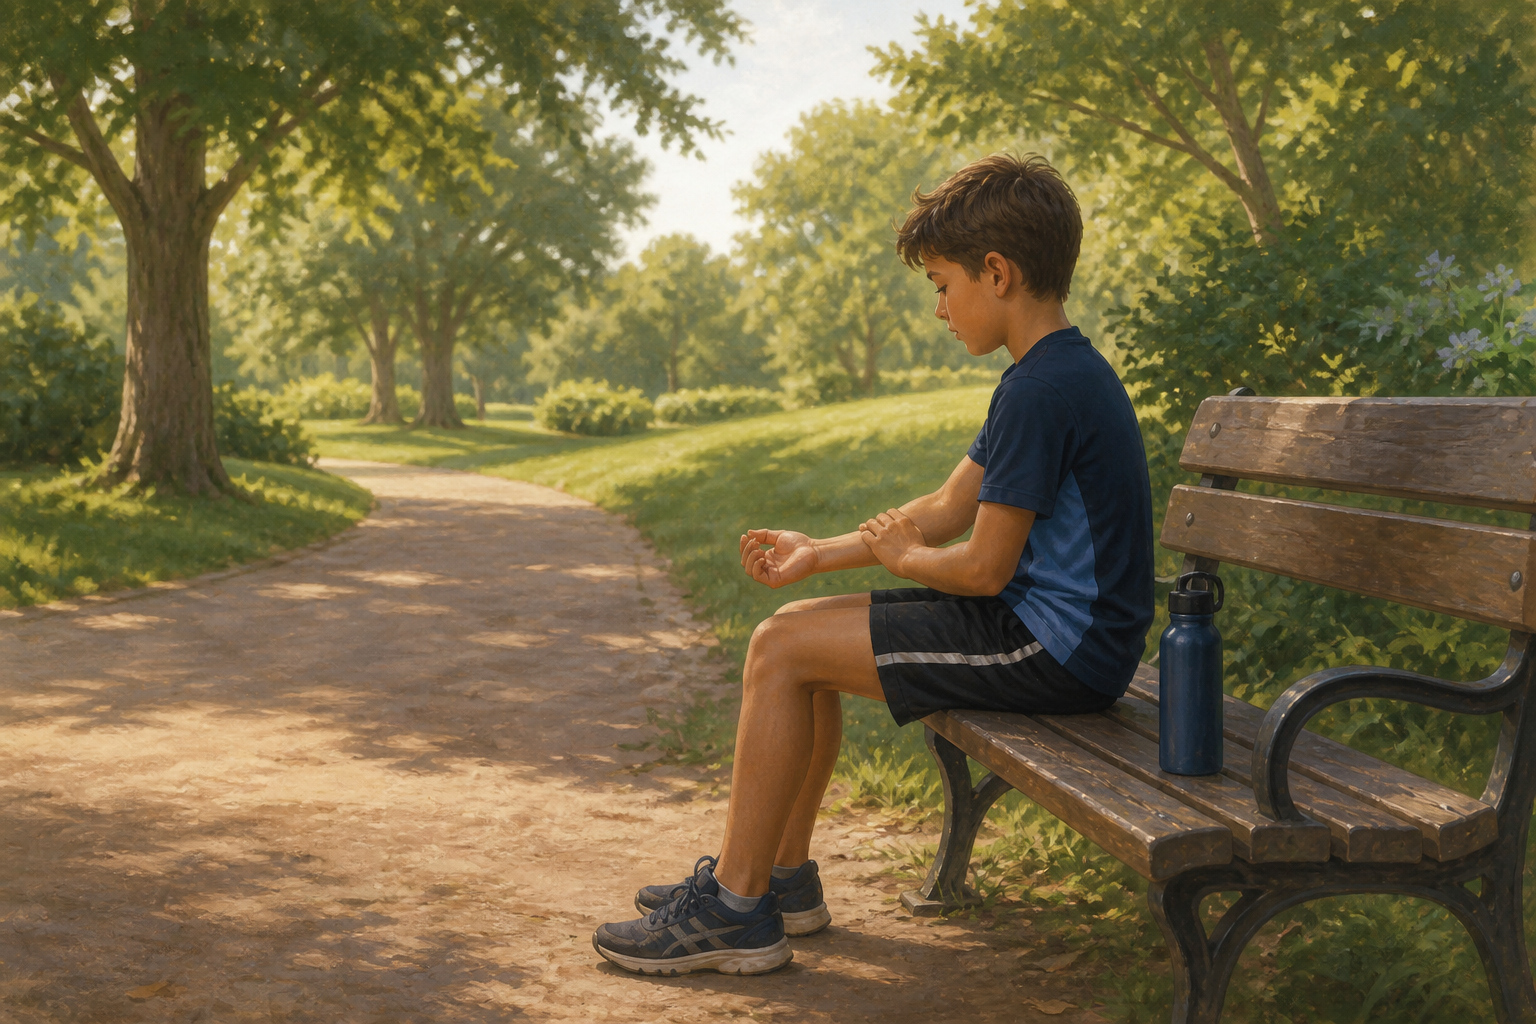
\includegraphics[width=0.58\linewidth]{images/book1/ai/g4-heart-rest.png}

{\small Sesudah berlari: dua jari di \omterm{def:g1:my-body:joint}{pergelangan tangan}, menghitung
pacuan \omterm{def:g4:heart-and-blood:heart}{jantungnya} dari kejauhan.}
\end{omfigure}

\begin{remark}[Otot yang tidak pernah beristirahat --- hampir]\label{rem:g4:heart-and-blood:rest}
Di antara dua denyut, \omterm{def:g4:heart-and-blood:heart}{jantungnya} mengendur selama sepersekian detik
--- serpihan itulah satu-satunya istirahat yang pernah diambilnya.
Siang dan malam, kira-kira $100000$ denyut sehari, seumur hidup.
Seperti setiap \omterm{def:g3:bones-and-muscles:muscle}{otot} (\cref{met:g3:bones-and-muscles:care}), ia menjadi
lebih kuat dengan latihan: \omterm{def:g4:heart-and-blood:heart}{jantung} yang terlatih memindahkan lebih
banyak \omterm{prop:g4:journey-of-food:absorb}{darah} tiap denyut, sehingga dapat berdenyut lebih tenang.
\end{remark}

\section{Latihan}

\begin{exercise}[$\star$]\label{exo:g4:heart-and-blood:1}
Sebutkan dua hal yang diantarkan \omterm{prop:g4:journey-of-food:absorb}{darah}, dan di mana ia memungut
masing-masing.
\end{exercise}

\begin{exercise}[$\star$]\label{exo:g4:heart-and-blood:2}
Gas buangan apa yang diangkut pergi oleh \omterm{prop:g4:journey-of-food:absorb}{darah}, dan di mana ia
menurunkannya?
\end{exercise}

\begin{exercise}[$\star$]\label{exo:g4:heart-and-blood:3}
\omterm{def:g4:heart-and-blood:heart}{Jantung} terbuat dari apa, seberapa besar ia, dan di mana ia duduk?
\end{exercise}

\begin{exercise}[$\star$]\label{exo:g4:heart-and-blood:4}
Apa yang dikerjakan tiap sisi \omterm{def:g4:heart-and-blood:heart}{jantung}?
\end{exercise}

\begin{exercise}[$\star$]\label{exo:g4:heart-and-blood:5}
Apa itu \omterm{prop:g4:heart-and-blood:pulse}{denyut nadi}, dan apa yang diberitahukan penghitungannya
kepadamu?
\end{exercise}

\begin{exercise}[$\star$]\label{exo:g4:heart-and-blood:6}
Mengapa \omterm{prop:g4:heart-and-blood:pulse}{denyut nadi} harus diukur dengan jari dan bukan dengan ibu
jari?
\end{exercise}

\begin{exercise}[$\star$]\label{exo:g4:heart-and-blood:7}
Mengapa \omterm{prop:g4:heart-and-blood:pulse}{denyut nadi} berpacu ketika berlari cepat? Ceritakan kisahnya
dari sudut pandang \omterm{def:g3:bones-and-muscles:muscle}{otot} \omterm{def:g1:my-body:parts}{tungkainya}.
\end{exercise}

\begin{exercise}[$\star$]\label{exo:g4:heart-and-blood:8}
Cobalah: ukurlah denyut nadimu ketika beristirahat dengan
\cref{met:g4:heart-and-blood:pulse}, lakukan lompatan bintang selama
tiga puluh detik, lalu ukurlah lagi. Laporkan kedua bilangannya.
\end{exercise}

\begin{exercise}[$\star\star$]\label{exo:g4:heart-and-blood:9}
Pada \cref{ex:g4:heart-and-blood:round}, tetes \omterm{prop:g4:journey-of-food:absorb}{darahnya} merah cerah
ketika meninggalkan \omterm{def:g4:breathing:organs}{paru-paru} dan lebih gelap ketika meninggalkan \omterm{def:g3:bones-and-muscles:muscle}{otot}
\omterm{def:g1:my-body:parts}{tungkainya}. Apa yang berubah padanya, pada tiap kalinya?
\end{exercise}

\begin{exercise}[$\star\star$]\label{exo:g4:heart-and-blood:10}
\omterm{prop:g4:journey-of-food:absorb}{Darah} menghubungkan tiga organ tahun ini: \omterm{def:g4:journey-of-food:tract}{usus halus}, \omterm{def:g4:breathing:organs}{paru-paru},
\omterm{def:g4:heart-and-blood:heart}{jantung}. Gambarkan atau lukiskan jaringannya: apa sumbangan
masing-masing bagi layanan pengantarannya?
\end{exercise}

\begin{exercise}[$\star\star\star$]\label{exo:g4:heart-and-blood:11}
\omterm{prop:g4:heart-and-blood:pulse}{Denyut nadi} istirahat seorang pengendara sepeda yang terlatih dapat
$50$; denyut orang dewasa yang tidak terlatih, $75$. Dengan memakai
\cref{rem:g4:heart-and-blood:rest}, jelaskan bagaimana \emph{lebih
lambat} dapat berarti \emph{lebih kuat} --- tiap denyut sang
pengendara sepeda pasti sedang mengerjakan apa?
\end{exercise}
